\documentclass[tikz,border=10pt]{standalone}
\usepackage{amsmath}
\begin{document}
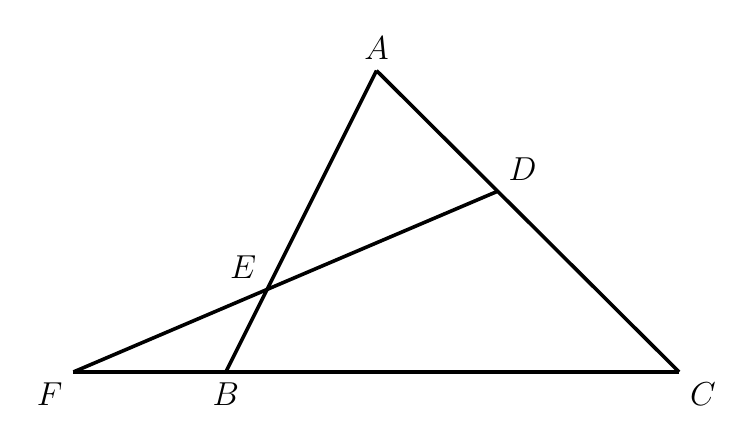
\begin{tikzpicture}[line join=round, line width=1.3pt]
\coordinate (A) at (-0.005,1.916);
\coordinate (B) at (-1.919,-1.911);
\coordinate (C) at (3.837,-1.911);
\coordinate (D) at (1.533,0.384);
\coordinate (E) at (-1.395,-0.863);
\coordinate (F) at (-3.854,-1.911);




\draw (F) -- (B) -- (C);


\draw (A) -- (D) -- (C);


\draw (A) -- (E) -- (B);


\draw (F) -- (E) -- (D);


\node[above] at (A) {\fontsize{13}{15.6}\selectfont $A$};
\node[below] at (B) {\fontsize{13}{15.6}\selectfont $B$};
\node[below right] at (C) {\fontsize{13}{15.6}\selectfont $C$};
\node[above right] at (D) {\fontsize{13}{15.6}\selectfont $D$};
\node[above left] at (E) {\fontsize{13}{15.6}\selectfont $E$};
\node[below left] at (F) {\fontsize{13}{15.6}\selectfont $F$};
\end{tikzpicture}
\end{document}